
\documentclass[11pt, a4paper]{book}
\usepackage{svn-multi}
\svnid{$Id$}
\usepackage{prelim2e}
\renewcommand{\PrelimWords}{Draft Copy \svnkw{Id}}
%%\newcommand*{\mysvnrev}{\svnrev}
\usepackage[hyperindex=true,
		   bookmarks=true,
            pdftitle={}, pdfauthor={Xi Yang},
            colorlinks=false,
            pdfborder=0,
            pagebackref=false,
            citecolor=blue,
            plainpages=false,
            pdfpagelabels,
            pagebackref=true,
            hyperfootnotes=false]{hyperref}
\usepackage[all]{hypcap}
\usepackage[palatino]{anuthesis}
\usepackage{afterpage}
\usepackage{graphicx}
\usepackage{thesis}
\usepackage[square]{natbib}
\usepackage[normalem]{ulem}
\usepackage[table]{xcolor}
\usepackage{makeidx}
\usepackage{cleveref}
\usepackage[centerlast]{caption2}
\usepackage{float}
\urlstyle{sf}
\renewcommand{\sfdefault}{uop}
\usepackage[T1]{fontenc}
\usepackage[scaled]{beramono}

\usepackage{multirow}


\renewcommand*{\backref}[1]{}
\renewcommand*{\backrefalt}[4]{
  \ifcase #1 %
    %
  \or
    (cited on page #2)%
  \else
    (cited on pages #2)%
  \fi
}




%      $Id: macros.tex 506 2009-10-05 16:57:07Z daniel $    

\usepackage{booktabs}
\usepackage{relsize}
\usepackage{xspace}
\usepackage{subfigure}
\usepackage{listings}
\lstloadlanguages{java}
\DeclareGraphicsRule{*}{pdf}{*}{}
\newcommand{\otoprule}{\midrule[\heavyrulewidth]}
\newcommand{\pldi}{ACM Programming Language Design and Implementation (PLDI)}
\newcommand{\taco}{ACM Transactions on Architecture and Code Optimization (TACO)}
\newcommand{\lctes}{ACM Languages, Compiler, and Tool Support for Embedded Systems (LCTES)}
\newcommand{\popl}{ACM Principles of Programming Languages (POPL)}
\newcommand{\ecoop}{European Conference for Object-Oriented Programming (ECOOP)}
\newcommand{\asplos}{ACM Architectural Support for Programming Languages and Operating Systems (ASPLOS)}
\newcommand{\sigmetrics}{ACM Measurement and Modeling of Computer Systems (SIGMETRICS)}
\newcommand{\oopsla}{ACM Object-Oriented Programming, Systems, Languages, and Applications (OOPSLA)}
\newcommand{\ismm}{International Symposium on Memory Management (ISMM)}
\newcommand{\veee}{ACM/USENIX Virtual Execution Environments (VEE)}
\newcommand{\micro}{ACM/IEEE International Symposium on Microarchitecture}
\newcommand{\isca}{ACM/IEEE International Symposium on Computer Architecture (ISCA)}
\newcommand{\icse}{International Conference  on Software Engineering (ICSE)}
\newcommand{\pact}{Parallel Architectures and Compilation Techniques (PACT)}
\newcommand{\casess}{ACM Compilers, Architectures, and Synthesis for Embedded Systems (CASES)}

\definecolor{tableheadcolor}{rgb}{0.8,0.8,1.0}
%\definecolor{tablealtcolor}{rgb}{0.9,0.9,1.0}
\definecolor{tablealtcolor}{rgb}{0.9,0.9,0.95}


\definecolor{todocolor}{rgb}{0.8,0.8,1.0}
\definecolor{fixcolor}{rgb}{1,0.8,0.8}
\definecolor{commentcolor}{rgb}{0.8,1.0,0.8}


\newcommand{\listingfigure}[3]{
\begin{figure}[ht!]
  \begin{center}
    \begin{minipage}[t]{\textwidth-4cm}
      \lstinputlisting{#1}
    \end{minipage}
  \end{center}
  \caption{#3}#2
\end{figure}}

\newcommand{\includeabchart}[5]{
\begin{figure}[ht!]
\begin{center}
\newcommand{\atitle}{#4}
\newcommand{\btitle}{#5}
\input{charts/#1.tex}
\end{center}
\caption{#3}#2
\end{figure}}

\newcommand{\placeholderfigure}[2]{
\begin{figure}[ht!]
  \begin{center}
    \resizebox{\textwidth-2cm}{0.7\textwidth-1.4cm}{todo}
  \end{center}
  \caption{#2}#1
\end{figure}}

\newcommand{\singlegraphfigure}[3]{
\begin{figure}[ht!]
  \begin{center}
    \includegraphics[width=\textwidth-2cm]{#1}
  \end{center}
  \caption{#3}#2
\end{figure}}

\usepackage[color=todocolor, colorinlistoftodos]{todonotes}

%\newcommand{\notinpart}{%
% \def\toclevel@chapter{-1}\def\toclevel@section{0}\def\toclevel@subsection{1}} \newcommand{\inpart}{
% \def\toclevel@chapter{0}\def\toclevel@section{1}\def\toclevel@subsection{2}}


%
% Stuff for pretty printing the source code using listings.sty
%


%% set Java as the default language
\lstset{
  numbers=left,
  numberstyle=\tiny,
  stepnumber=1,
  numbersep=2em,
  language=java,                         % the language
  basicstyle=\footnotesize\ttfamily,     % the basic font family to use
  commentstyle=\itshape,                 % the font for comments
  stringstyle=\ttfamily,
%  morekeywords={@Intrinsic, @Unboxed, @RawStorage}
}
%\lstset{language=java}

\newcommand{\textjava}[1]{{\lstset{basicstyle=\ttfamily}\lstinline@#1@}}
\newcommand{\textjavafn}[1]{{\lstset{basicstyle=\footnotesize\ttfamily}\lstinline@#1@}}
%\usepackage{lstasm}
\usepackage{setspace}
\usepackage{ifthen}
%\usepackage{color}
%\usepackage{smallheadings}

\long\def\sfootnote[#1]#2{\begingroup%
\def\thefootnote{\fnsymbol{footnote}}\footnote[#1]{#2}\endgroup}
%
% code
%

\newcommand{\address}{\textjava{Address}\xspace}
\newcommand{\ubregion}{\textjava{unbump-region()}\xspace}
\newcommand{\word}{\textjava{Word}\xspace}
\newcommand{\freeme}{\textjava{free()}\xspace}
\newcommand{\freemeunbump}{\textjava{unbump()}\xspace}
\newcommand{\freemeunbumpregion}{\textjava{unbump-region()}\xspace}
\newcommand{\freemeunreserve}{\textjava{unreserve()}\xspace}

%
% abbreviations
%


\newcommand{\eg}{e.g., }
\newcommand{\ie}{i.e., }

\newcommand{\GenMS}{\emph{GenMS}\xspace}
\newcommand{\GenImmix}{\emph{GenIX}\xspace}
\newcommand{\mmtk}{MMTk\xspace}
\newcommand{\jikes}{Jikes RVM\xspace} 
\newcommand{\jikesrvm}{\jikes} 
\newcommand{\jala}{Jalape\~{n}o\xspace} 
\newcommand{\jalapeno}{Jalape\~{n}o\xspace} 

\newcommand{\dacapo}{\textsf{DaCapo}\xspace}
\newcommand{\specjvm}{\textsf{SPECjvm98}\xspace}
\newcommand{\cattrack}{\textsf{cattrack}\xspace}
\newcommand{\spec}{\textsf{SPEC}\xspace}

\newcommand{\nurserytype}[1]{{\fontfamily{cmss}\selectfont \textsl{#1}}}
\newcommand{\alloc}{\nurserytype{allocate}\xspace}
\newcommand{\collect}{\nurserytype{collect}\xspace}
\newcommand{\redirect}{\nurserytype{redirect}\xspace}

\newcommand{\bmtype}[1]{{\textsf{#1}}}

\newcommand{\jbb}{\bmtype{jbb2000}\xspace}
\newcommand{\psjbb}{\bmtype{pjbb2005}\xspace}
\newcommand{\pjbb}{\bmtype{pjbb2005}\xspace}
\newcommand{\specjbb}{\bmtype{SPECjbb2005}\xspace}
\newcommand{\jess}{\bmtype{jess}\xspace}
\newcommand{\raytrace}{\bmtype{raytrace}\xspace}
\newcommand{\db}{\bmtype{db}\xspace}
\newcommand{\javac}{\bmtype{javac}\xspace}
\newcommand{\jack}{\bmtype{jack}\xspace}
\newcommand{\compress}{\bmtype{compress}\xspace}
\newcommand{\mpegaudio}{\bmtype{mpegaudio}\xspace}
\newcommand{\mtrt}{\bmtype{mtrt}\xspace}
\newcommand{\antlr}{\bmtype{antlr}\xspace}
\newcommand{\bloat}{\bmtype{bloat}\xspace}
\newcommand{\chart}{\bmtype{chart}\xspace}
\newcommand{\eclipse}{\bmtype{eclipse}\xspace}
\newcommand{\fop}{\bmtype{fop}\xspace}
\newcommand{\hsqldb}{\bmtype{hsqldb}\xspace}
\newcommand{\jython}{\bmtype{jython}\xspace}
\newcommand{\luindex}{\bmtype{luindex}\xspace}
\newcommand{\lusearch}{\bmtype{lusearch}\xspace}
\newcommand{\Lusearch}{\bmtype{Lusearch}\xspace}
\newcommand{\pmd}{\bmtype{pmd}\xspace}
\newcommand{\ps}{\bmtype{ps}\xspace}
\newcommand{\SPECjbb}{\bmtype{SPECjbb}\xspace}
\newcommand{\xalan}{\bmtype{xalan}\xspace}
\newcommand{\sunflow}{\bmtype{sunflow}\xspace}
\newcommand{\Sunflow}{\bmtype{Sunflow}\xspace}
\newcommand{\avrora}{\bmtype{avrora}\xspace}
\newcommand{\core}{Core2 Quad\xspace}
\newcommand{\corelong}{Intel Core2 Quad Q6600\xspace}
\newcommand{\phenom}{Phenom II\xspace}
\newcommand{\phenomlong}{AMD Phenom II X6 1055T\xspace}
\newcommand{\sandy}{i7-2600\xspace}
\newcommand{\sandylong}{Intel Core i7-2600\xspace}



\newcommand{\ghostscript}{\bmtype{ghostscript}\xspace}

\newcommand{\doi}[1]{\href{http://dx.doi.org/#1}{\nolinkurl{doi:#1}}}
%
% misc
%
\newcommand{\fix}[1]{\todo[color=fixcolor]{#1}}
\newcommand{\comment}[1]{\todo[color=commentcolor]{#1}}
\newcommand{\ifix}[1]{\todo[inline,color=fixcolor]{#1}}
\newcommand{\icomment}[1]{\todo[inline,color=commentcolor]{#1}}
\newcommand{\itodo}[1]{\todo[inline]{#1}}
\newcommand{\ignore}[1]{}
\newcommand{\mccenter}[1]{\multicolumn{1}{c|}{#1}}

%
% figure spacing
%
%\clubpenalty 10000
%\widowpenalty 10000
%\def\topfraction{0.9}
%\def\bottomfraction{0.9}
%\def\textfraction{0.1}
%\renewcommand{\singlespacing}{\renewcommand{\baselinestretch}{1.00}\small\normalsize}
%\renewcommand{\doublespacing}{\renewcommand{\baselinestretch}{1.5}\small\normalsize}
%\newcommand{\tight}{\renewcommand{\baselinestretch}{1.28}\small\normalsize}
%\renewcommand{\subfigbottomskip}{0.25ex}
%\renewcommand{\subfigcapskip}{0ex}
%\renewcommand{\subfigcapskip}{-1ex}
%\newcommand{\subfigshrink}{-0.75ex}
%\newcommand{\subfigcapspace}{2ex}

%\newcommand{\subwidth}[0]{.32\textwidth}


%
% margins
%
%\topmargin -.5truein
%\textheight 9truein
%\oddsidemargin .25truein
%\evensidemargin .25truein
%\textwidth 6truein


%
% crossreferencing footnotes
%
%\newcommand{\fnref}[1]{~(\ref{#1})}
%\newcommand{\onecolparbox}{3.1in}


%\newcommand{\textjava}[1]{{\lstset{language=java,basicstyle=\footnotesize\ttfamily}\lstinline@#1@}}
%\newcommand{\textasm}[1]{{\lstset{language=asm,basicstyle=\footnotesize\ttfamily}\lstinline@#1@}}

%%
%% Change the sections etc.
%%
%\makeatletter
%\parskip=0pt
%\renewcommand\section{\@startsection{section}{1}{\z@}%
%                                   {-2.5ex}% beforeskip
%%                                   {1ex}% afterskip
%                                   {\large \bfseries \raggedright}}
% \renewcommand\subsection{\@startsection{subsection}{2}{\z@}%
%                                     {-2ex\@plus -1ex \@minus -.2ex}%
%                                      {.5ex \@plus .2ex}%
%                                      {\normalsize \bfseries \raggedright}}
% \renewcommand\subsubsection{\@startsection{subsubsection}{3}{\z@}%
%                                      {-2ex\@plus -1ex \@minus -.2ex}%
%                                      {1ex \@plus .2ex}%
%                                      {\normalfont\fontsize{11pt}{12pt}\selectfont\itshape}}
%\renewcommand{\thesubsubsection}{\thesubsection.\arabic{subsubsection}}

%\renewcommand\paragraph{\@startsection{paragraph}{4}{\z@}% 
%  {.5em}%
%  {-1em}%
%  {\normalfont\normalsize\bfseries\parskip=0pt}}
%\setlength\partopsep{0\p@}
%\setlength\parskip{0\p@ \@plus \p@}

%\makeatother
%\parindent=9pt





%%% Local Variables: 
%%% mode: latex
%%% TeX-master: "doa"
%%% End:
            
%%%%%%%%%%%%%%%%%%%%%%%%%%%%%%%%%%%%%%%%%%%%%%%%%%%%%%%%%%%%%%%%%%%%%%%
%% Preamble
\title{Formally Verified Electronic Voting Scheme : A Case Study}
\author{Mukesh Tiwari}
\date{\today}

\renewcommand{\thepage}{\roman{page}}

\makeindex
\begin{document}
%\doparttoc
%%%%%%%%%%%%%%%%%%%%%%%%%%%%%%%%%%%%%%%%%%%%%%%%%%%%%%%%%%%%%%%%%%%%%%%
%% Title page
\pagestyle{empty}
\thispagestyle{empty}
%% anuthesis.sty Copyright (C) 1996, 1997 Steve Blackburn
%% Department of Computer Science, Australian National University
%%

\begin{titlepage}
  \enlargethispage{2cm}
  \begin{center}
    \makeatletter
    \Huge\textbf{\@title} \\[.4cm]
    \Huge\textbf{\thesisqualifier} \\[2.5cm]
    \huge\textbf{\@author} \\[9cm]
    \makeatother
%%   \LARGE A thesis submitted for the degree of \\
%%    Master of Philosophy at \\
%%    The Australian National University \\[2cm]
    \LARGE A thesis submitted for the degree of \\
    YOUR DEGREE NAME \\
    The Australian National University \\[2cm]
    \thismonth
  \end{center}
\end{titlepage}


%%%%%%%%%%%%%%%%%%%%%%%%%%%%%%%%%%%%%%%%%%%%%%%%%%%%%%%%%%%%%%%%%%%%%%%
%% Here begin the preliminaries
\vspace*{14cm}
\begin{center}
  \makeatletter
  \copyright\ \@author{} 2011
  \makeatother
\end{center}
\noindent
\begin{center}
  \footnotesize{~} %\aboutthesis
\end{center}
\noindent

\newpage

\vspace*{7cm}
\begin{center}
  Except where otherwise indicated, this thesis is my own original
  work.
\end{center}

\vspace*{4cm}

\hspace{8cm}\makeatletter\@author\makeatother\par
\hspace{8cm}\today


%%%%%%%%%%%%%%%%%%%%%%%%%%%%%%%%%%%%%%%%%%%%%%%%%%%%%%%%%%%%%%%%%%%%%%%
%% Dedication
\cleardoublepage
\pagestyle{empty}
\vspace*{7cm}
\begin{center}
To my grandparents, who despite being a poor farmer, understood the value of education.
\end{center}


%%%%%%%%%%%%%%%%%%%%%%%%%%%%%%%%%%%%%%%%%%%%%%%%%%%%%%%%%%%%%%%%%%%%%%%
%% Acknowledgements
\cleardoublepage
\pagestyle{empty}
\chapter*{Acknowledgments}
\addcontentsline{toc}{chapter}{Acknowledgments}
This thesis could not have been possible without the support of my supervisor, Dirk Pattinson. I really 
admire this abilities and intuition to make sure that I stay clear from many dead ends. Moreover, 
I thank him for patiently answering my stupid questions happily and guiding me towards the right 
answer by asking the right questions. My only wish to be researcher like 
him and incorporate more of his qualities, but I am less optimistic about my chance. 

I also want to thank my dog Turbo who would patiently listen to my proofs
and ideas about my PhD with occasionally barking at me if he was bored of listening. He truly made my PhD a breeze, 
and I never felt pressure of PhD when I was walking with him. 

I want to thank Optus, Australian Mobile Service Provider, for launching unlimited calling scheme to India. 
Because of this scheme, I was able to talk to my mom everyday by normal call because she does not know how 
to operate a smart phone. 
 
Some of the great friends who made this journey possible are Caitlin D'Abrera, Milad Ketab Ghale Ali,  Jim De Groot, 
Ian Shillito (my occasional philosophy discussion partner), Ali Cheraghian, and Ahmad Attarha. Although, 
 their lunch time adult jokes were too much for me to digest, but I enjoyed it whenever I could.  
 
 I learned many valuable things 
 from Micheal during the thesis presentation which helped me shaping my personality and how to present it. 
 
 I want to thank Thomas Haines, my co-author,  for teaching me all the bits pieces of cryptography. I really 
 enjoyed working with him. 
 
 One of the best experience of this PhD was travelling to Princeton to participate in summer. 
 Unfortunately, I could not attend Marktoberdorf because it was impossible for me to get the visa of Germany, but I hope
 things would be more easier in the upcoming future. 
 
 Last and above all, I want to thank Mina. Being by your side for the last two years has been the best thing that ever happened to me, and I could not 
 imagine life without you.   I am also grateful to all the efforts you made to bear my tendencies to constantly
  talk about set-theory/formal-verification/every-thing-except-romantic.

 Last, but not least, the good wine and beer of Australia could not go unmentioned in this PhD. 
One of the biggest joy of this PhD was to meet my girlfriend, Mina, who came as a visitor to our logic group. 


%%%%%%%%%%%%%%%%%%%%%%%%%%%%%%%%%%%%%%%%%%%%%%%%%%%%%%%%%%%%%%%%%%%%%%%
%% Abstract
\cleardoublepage
\pagestyle{headings}
\chapter*{Abstract}
\setlength{\parindent}{2em}
\setlength{\parskip}{1em}
\addcontentsline{toc}{chapter}{Abstract}

%\vspace{-1em}


Since the introduction of secret ballots in Victoria, Australia in 1855, 
paper (ballots) are widely used around the world to record 
the preferences of eligible voters. Paper ballots provide three 
important ingredients: correctness, privacy, and verifiability. 
However, the paper ballot election brings various  other challenges, e.g. 
it is slow for large democracies like India,  and error prone for complex voting method 
like single transferable vote, and poses operational challenges for 
large countries like Australia. In order to solve these problems and various others, 
many countries are adopting electronic voting. However, 
electronic voting has a whole new set of problems. In most cases, the software 
programs used to conduct the election have numerous problems, including, but no limited to, 
counting bugs, ballot identification, etc. Moreover, 
these software programs are treated as commercial in confidence and 
are not allowed to be inspected by members of the public. 
As a consequence, the result produced by these software programs 
can not be substantiated.

In this thesis, we address the three main concerns posed by electronic voting, i.e. 
correctness, privacy, and verifiability. We address the correctness concern by using 
theorem prover to implement the vote counting algorithm, 
privacy concern by using  cryptography,  and verifiability concern 
by generating a independently checkable scrutiny sheet (certificate). Our work 
has been carried out in the Coq theorem prover.

%%% Local Variables: 
%%% mode: latex
%%% TeX-master: "paper"
%%% End: 

%%%%%%%%%%%%%%%%%%%%%%%%%%%%%%%%%%%%%%%%%%%%%%%%%%%%%%%%%%%%%%%%%%%%%%%
%% Table of contents
\cleardoublepage
\pagestyle{headings}
\markboth{Contents}{Contents}
\tableofcontents
\listoffigures
\listoftables

%%%%%%%%%%%%%%%%%%%%%%%%%%%%%%%%%%%%%%%%%%%%%%%%%%%%%%%%%%%%%%%%%%%%%%
%% Here begins the main text
\mainmatter

%% Introduction
\chapter{Introduction}
\label{cha:intro}
\epigraph{The best weapon of a dictatorship is secrecy, but the best weapon of a democracy should be the weapon of openness.} 
{\textit{Niels Bohr}} 

\section{Problem Statement}

A democracy can be described as a system where all eligible voters have equal rights to express their opinion(s) on different matters. 
One of the most important example of expressing the opinion is holding elections to elect the leader of country. During the 
elections, all eligible voters express their opinion on a paper, also known as ballot,	 in a manner, depending on the voting method, 
which reflects their true opinion. For example, if the voting method is \textit{ranked voting (preferential voting)}, then the voters rank the 
candidates according to their preference, and if the method is \textit{first past the post}, then each voter selects one candidate by marking
against the candidate name in the ballot. Later, once the ballot cast finishes, a candidate is elected as a winner from  the participating
candidates by combing the choices of all the voters. 
The paper ballot method works great, except it is very time consuming, expensive, error prone, 
and not very inclusive for disabled voters such as visually impaired.
In order to solve the various problems posed by paper ballot, many countries are adopting electronic voting as an alternative. 
Electronic voting is 
getting popular in many countries, and the reason for its popularity is cost-effective, faster result, high voter turn out, 
and accessible for disabled voters.  
Undeniably, electronic voting has helped, for example, Australia to ease the logistic challenges of elections because of its massive land size and sparsely 
population and save millions of dollars.  In addition, it has helped India, the second most populous country with 900 million eligible voter, to declare 
2019 election with 67 percent voter turn out (roughly 600 million) in 2 days, and  Estonia, a labour shortage country, has saved 
thousands of man hours, 11,000 working days, by using electronic voting \citep{Estonia}.

   
  Despite all these benefits, electronic voting is an arduous effort because a minuscule possibility of 
  going anything wrong in software or hardware could lead to a disaster,   possibly 
  inverting the results \citep{TSwiss},
  \citep{10.1007/978-3-319-22270-7_3}, \citep{ARANHA2019335},
  \citep{Feldman:2007:SAD:1323111.1323113}.  The nature of (electronic) data and ease of 
  its manipulability/misinterpretation causes electronic voting many problems, which are not present in paper ballot elections, that 
  makes it perfectly susceptible to delivering wrong and unverifiable result \citep{Wolchok:2010:SAI:1866307.1866309}.
  For instance,  if a software program used in electronic voting 
  for reading the ballots has byte order bug, or even if it depends on some other software which has byte order bug (the data is suppose to read 
  from left to right, but software is reading right to left), then the interpretation of 
  ballot would completely be different from what the voter had in mind.
  More often than not, these software programs are configured incorrectly \citep{1301313} and run at the top of (untrusted) operating 
  system and hardware. Usually, operating systems have millions of lines code (Linux has 15 millions lines) which exposes
  a large attack surface and could be exploit, possibly by current government or foreign countries, for illegal gain.
  The worst, these software and hardware  are commercial in 
  confidence and treated as a black-box, and, most often, their source code or design is not open 
  for public scrutiny \citep{AEC:2013:LMM}. In addition, these software programs 
  take a list of ballots and produce the result without producing any evidence about the correctness of result.  As a consequence,
  from casting the ballot electronically and declaring winner based on cast (electronic) ballot, the whole process lacks basic assumptions
  of democracy such as transparency, genuineness, and verifiability. 
  
  In order to make the electronic voting process genuine and trustworthy, electronic voting 
  research community has recognized some must have properties of electronic voting protocol
  \citep{5958051}, 
   \citep{Benaloh:1994:RSE:195058.195407},  \citep{Delaune:2010:VPT}, \citep{Bernhard:2017:PES}:
  

 \begin{itemize}
 
  \item Correctness:
 	The produced results are correct, and convincing to all leaving no  ground for suspicion. 

 \item Coercion-resistance: A voter can not cooperate with a coercer to prove anything about her choices.
 
 \item Eligibility: Only eligible voter can cast the ballot.
 	
 \item Privacy:
    All the votes must be secret, and voter should not be able to convince anyone the 
    value of her vote.
 
 \item End-to-end Verifiability:
 Any independent third party should be able to verify the final outcome of election based on cast 
 ballots.  It can be further divided into three sub-categories:
 
 \begin{itemize}
  \item Cast-as-intended: Every voter can verify that their ballot was cast as
  intended.
  \item Collected-as-cast: Every voter can verify that their ballot was collected as
  cast.
  \item Tallied-as-cast: Everyone can verify final result on the basis of the
  collected ballots.
\end{itemize}
\end{itemize}
	

In this thesis, we focus on privacy, correctness, coercion-resistance, and tallied-as-cast, the third part of end-to-end verifiability, property 
of an election. Furthermore, we assume that the first two properties of end-to-end verifiability, \textit{cast-as-intended} and 
\textit{collected-as-cast}, hold for an election. \textit{Cast-as-intended} is a verification method that is used to audit the 
front end voting software, 
also known as voting client software, to make sure that it is not modifying the options of voters. In a nutshell, 
the cast-as-intended is assurance to a voter that front-end software is transparent and her vote 
is recorded according to her intent.  \textit{Cast-as-intended} is itself an active area of research in its own right; 
however, it is not the focus of this thesis. Similarly, \textit{Collect-as-cast} is a notion related to the voters to make 
sure that the ballots appearing on the bulletin board are indeed the ballots that cast during the election. A consequence 
of \textit{collected-as-cast} notion is that any attempt to change or delete the ballots from the bulletin board would 
be detected. This notion is indeed a crucial one and works as a bridge between cast-as-intended and tallied-as-cast 
notion. However, it is related to voters' behaviour; hence, the reason for assumption.  Moreover, assuming these two 
notions, cast-as-intended and collected-as-cast, helped us in isolating the irrelevant details and 
paved a way to focus on more complex problem of counting, i.e. tallied-as-cast. 


\section{Research Motivation and Contribution}
Given the potential advantages of electronic voting,  we need to address
the correctness, privacy, and verifiability concerns for its widespread adoption. 
This thesis sets out to address these concerns of electronic voting. 
The questions we asked ourself was:
 \begin{enumerate} 
  \item Can we implement a vote counting protocol with the  
    "guaranteed" correctness
    of the implementation and practical enough
    to count the real life election involving millions of ballots (Correctness)?
  \item Can we produce the result by counting encrypted ballot without revealing 
  its content, and at the same time, 
  assuring everyone that the result produced is only based on "valid" ballots, 
  and "invalid" ones have been discarded  (Privacy and Coercion-resistance)?
 \item Can we decouple the verifiability from implementation, i.e. 
    generating enough evidence so that any independent auditor can 
    ascertain the outcome of election without trusting the implementation 
    of software used to conduct the election (Verifiability)?
  \end{enumerate}


In order to answer these questions, at first we need two things: (i) a voting protocol and 
(ii) a tool to implement the voting protocol and prove the correctness properties of the implementation. 
Our choice of voting protocol is the   Schulze method \citep{Schulze:2011:NMC} and 
the tool is Coq \citep{Bertot:2004:ITP} theorem prover  for implementing and proving 
the correctness of  Schulze method.
Even though Schulze method is not used in any democratic election to public office,
it has many interesting properties and, 
 at the same time, it is non-trivial.  
While no preferential voting scheme can guarantee all desirable properties that one would
like to impose due to Arrow’s theorem \citep{Arrow:1950:DCS}, the Schulze method offers a good compromise, 
with a number of important properties already  established  in  Schulze’s  original  paper. 
Amongst the various  properties, Schulze method satisfies the \textit{resolvability criterion}, 
i.e. elects a single winner under the assumption that number of voters are much larger than
 number of candidates (and in case of tie, when there are more than one winner, a random vote can be 
selected to declare winner.  However, our formalization 
has not taken the randomness into account, so it can produce more than one winner). 
Coq is a theorem prover (proof assistant) based on \textit{Calculus of Inductive Construction} 
\citep{Coquand:1988:CC:47724.47725} \citep{coquand1988inductively}. 
The \textit{Calculus of Inductive Construction} allows the "proof" terms and 
"computation" terms to live in the same universe (level), which leads to a highly expressive type 
system. Moreover, during the proof development, 
it provides a step by step feedback to the user and possibility to automate the proofs by 
writing the custom tactics using the Ltac \citep{10.5555/1765236.1765246}. In addition, 
Coq proofs can be extracted into the  Haskell, OCaml, and Scheme.
 
Now that we have a voting protocol (Schulze method) and  a tool (Coq theorem prover), 
we demonstrate that it is possible to achieve correctness, privacy, coercion-resistance, and (tallied-as-cast) verifiability in 
electronic voting. We achieve the following:
\begin{itemize}
 \item \textit{Correctness} by formally specifying the Schulze method  and prove its correctness properties
  inside the Coq theorem prover. 
 Coq has a well developed extraction facility that 
 we use to extract proofs into OCaml programs, and using these extracted OCaml programs, we 
 have counted the ballots from election to produce the result. 
 \item \textit{Privacy and Coercion-resistance} by encryption. We use homomorphic encryption to compute the 
  finally tally without decrypting any individual ballot. 
\item \textit{Verifiability} by tabulating the relevant data of election (we call it scrutiny-sheet/certificate).
   Achieving verifiability in a plain-text ballot counting is fairly straight forward.  
   To achieve verifiability in encrypted ballot counting, 
   we augment the scrutiny sheet with zero-knowledge-proof for the each claim we make during the 
   counting which can  later be checked by any auditor.  
\end{itemize}



In addition to demonstrating correctness, privacy and verifiability, we have also developed a formally verified certificate 
checker. Moreover, we have shown that our implementation adheres to the various properties established by Schulze in 
his original paper. 

\noindent 
\textit{Formally Verified Checker:} Third party independent election audit based on scrutiny sheet data is a crucial step towards 
establishing the trust in the system.   However, auditing the scrutiny sheet of an election involving encrypted ballots
is not straight forward in comparison to an election with plain-text ballots. 
In general, auditing the scrutiny sheet of an election involving 
plain-text ballot simply requires the knowledge of basic arithmetic, e.g. addition, subtraction and multiplication, 
and virtually anyone can audit the election based on the data produced in the scrutiny sheet by
using a calculator or by writing a simple program in her preferred language. 
However, encrypted ballot election scrutiny sheet involves various
cryptographic concepts (homomorphic encryption, zero knowledge proof, commitment scheme, etc.) 
which are accessible to a very few voters, mainly cryptographers,  so auditing it 
requires deep understanding of cryptographic principals. To ease this situation, we have developed a formally verified 
certificate checker as a proof of concept for automating the auditing an election conducted on encrypted ballots. 
Having said that,  our certificate generated by encrypted ballots is very complex, and formalizing all the cryptographic 
primitives involved would be fairly time consuming, so we have developed a proof of concept 
formally verified certificate checker for International Association of Cryptographic Research 2018 election
scrutiny sheet, relatively simple than ours. 

\noindent
\textit{Properties of Schulze Method:} We have proved couple of the properties, Condercet winner and Reversal symmetry, 
of the Schulze method inside Coq theorem prover (ongoing work).
 

\section{Cryptographic Blackbox}
Since the beginning of this project, our primary goal was 
to achieve privacy (using encryption) and verifiability (using zero knowledge proof) in electronic voting 
using the cryptographic primitives (but not the verification of primitives itself). 
To achieve this goal, we have 
taken the axiomatic approach and assumed the existence of cryptographic primitives 
inside Coq. Moreover, we assume the axioms about their correctness behaviour, e.g. 
decryption is left inverse of encryption. These primitives, in general, provide functionality 
of generating a random permutation, encrypting a plain-text, decrypting a cipher-text, 
producing commitment of a value, constructing a zero-knowledge-proof, 
and verifying a zero-knowledge-proof. Later, in extracted OCaml code from Coq code, these functions are instantiated 
with Unicrypt \citep{LocherH14} function. 
\footnote{Formalizing the whole cryptographic stack used in our 
project would be very time consuming (probably a PhD itself), but it would be worth trying. 
Although, we have formalized the (El-Gamal) encryption, and decryption inside Coq, but we still 
are very far from achieving the goal of fully verified cryptographic stack.  We leave the formalisation 
of cryptographic primitives for future work (work in progress).}



\section{Publication}
 The chapters, or some part of it,  of this thesis are based on the following papers:
	\begin{enumerate}
	\item Pattinson, D. and Tiwari, M., 2017. Schulze Voting as Evidence carrying computation. In Proc. 
	ITP 2017, vol. 10499 of Lecture Notes in Computer Science, 410–426. Springer. 
	\item Lyria Bennett Moses, Rajeev Goré, Ron Levy, Dirk Pattinson, Mukesh Tiwari.
	No More Excuses: Automated Synthesis of Practical and Verifiable Vote-Counting Programs for Complex 
	Voting 	Schemes. E-VOTE-ID 2017: 66-83
	\item Milad K. Ghale, Rajeev Goré, Dirk Pattinson, Mukesh Tiwari.
	Modular Formalisation and Verification of STV Algorithms. E-Vote-ID 2018: 51-66
	\item Thomas Haines, Dirk Pattinson, and Mukesh Tiwari. 2019. 
	  Verifiable Homomorphic Tallying for the Schulze Vote Counting Scheme. 
	  11th International Conference Verified Software: Theories, Tools, and Experiments. 
      VSTTE 2019 (to appear)	  
	\item Thomas Haines, Rajeev Goré, and Mukesh Tiwari. 2019. Verified Verifiers for Verifying Elections. 
	 In Proceedings of the 2019 ACM SIGSAC Conference on Computer and Communications Security (CCS '19).
	\end{enumerate}
 \noindent
 Part of chapter \ref{cha:background} is based on \textit{No More Excuses: Automated Synthesis of Practical 
 and Verifiable Vote-Counting Programs for Complex Voting  Schemes},
 chapter \ref{cha:schulze_method} is based on \textit{Schulze Voting as Evidence Carrying Computation},
 chapter \ref{cha:homormorphic_schulze} is based on \textit{Verifiable Homomorphic Tallying for the 
 Schulze Vote Counting Scheme}, and part of chapter
 \ref{cha:software_independence} is based on \textit{Verified Verifiers for Verifying Elections}.




\section{Related Work}
 There is extensive work that 
 addresses the different issues related of electronic voting protocols  in symbolic model, 
 but there are very few, to the best of my knowledge, 
 that have used theorem provers to implement the voting protocol (counting algorithm)
 and verify its correctness properties. 
 \citep{10.1007/978-3-540-31987-0_14}, and  \citep{Delaune2010} have used pi-calculus, a formalism for describing concurrent systems,
 to model and analyse various properties, such as fairness, eligibility, vote-privacy, receipt-freeness and 
 coercion-resistant,  
 of the protocol FOO developed by \citep{10.1007/3-540-57220-1_66}.  \citep{Backes:2008:AVR:1380848.1381255}
 presented a general technique to model  remote electronic 
 voting protocol and automatically verifying  its security properties using pi-calculus. 
 \citep{5992139} have used pi-calculus to analyse the ballot secrecy of \citep{Helios:2016:HVS}.
 \citep{10.1007/978-3-642-28641-4_7} have used pi-calculus to ascertain the properties of 
 Norwegian electronic voting protocol.
 \citep{10.1007/978-3-319-68687-5_7} have used Tamarin  to prove receipt-freeness 
 and vote-privacy of Selene voting protocol \citep{Selene}.  Most of these work differs from ours
 in the sense that their primary focus is verification of security protocol in  
 Dolev-Yao model or  complexity-theoretic model, whereas our work is 
 more focused on verified implementation and  verifiability  aspect of vote counting.

 The closest to our work is \citep{Cochran:2010:VFS} \citep{DeYoung:2012:LLV}, \citep{Pattinson:2015:VCM}, \citep{Pattinson:2016:MSP},
 \citep{Verity:2017:FVI:3014812.3014845}, and \citep{Ghale:2017:FVS}. \citep{Cochran:2010:VFS} have used
 Business Object Notation (BON) and Java Modelling Language (JML) to formally specify their 
 Java implementation of  Irish Proportional  Representation  by  Single  Transferable  Vote  (PR-STV) 
 method.  They relied on Extended Static Checking to validate the correctness of their 
 implementation. Upon further investigation \citep{Cochran:2013:FMB}, they improved it 
 by writing formal specification of  candidate, ballot, and ballot box datatypes 
 using the Alloy model checker \citep{10.1145/505145.505149}. However, they themselves pointed out that:
 \begin{displayquote}
 Note that this automated consistency checking is not the same as providing a 
 full interactive proof of a soundness theorem in a higher-order logical framework.
 Such formalization is an interesting and useful exercise, but we did not do it for this 
 case study. Instead, checking the dozens of theorem stipulated in law text is more 
 akin to the kind of validation that we are advocating in this work. 
 It gives us high confidence, but not a proof, that the mechanical formalization is
  sound and complete.
  \end{displayquote}
 
 \noindent
 \citep{DeYoung:2012:LLV} used linear logic \citep{GIRARD19871} to model the different entity in electronic voting as a resource. 
 The use of linear logic makes it very natural to capture the different entities in electronic voting,  
 depending on their usage, by means of modality e.g. a voter can cast only one vote, but she might 
 need to show her photo id to multiple times at counting booth. \citep{Pattinson:2015:VCM} treated 
 the process of vote counting from
 the perspective of mathematical proof. They used (mathematical) proof theory to model the 
 counting. \citep{Ghale:2017:FVS} have formalized single transferable vote in Coq and 
 extracted Haskell code from the formalization. The extracted Haskell code produces the result 
 and a certificate for a given set of input ballots. This certificate can be used by any third party to verify 
 or audit the outcome of election result.  However, none of these work considers privacy and coercion resistance as a key 
 issue in electronic voting, and their method simply works for plaintext ballots which are  susceptible to 
 italian attack  \citep{Otten}   \citep{Benaloh:2009:SSC}.

\section{Outline of the Chapters}
\begin{itemize}

\item Chapter \ref{cha:background} provides an overview of electronic voting around the world, 
problems in general, and rationale for formal verification of election voting software. 
\item Chapter \ref{cha:theorem_crypto} provides the overview of concept of 
Coq theorem prover  and cryptographic primitives.  
\item Chapter \ref{cha:schulze_method} 
describes Schulze method, its formal specification, proof of correctness, experimental result, 
and scrutiny sheet.  
\item Chapter \ref{cha:homormorphic_schulze} describes 
verifiable homomorphic tally for the Schulze method, its realization in theorem prover, experimental 
result,  instructions to audit the scrutiny sheet. 
\item Chapter \ref{cha:software_independence} focuses on the notion of software independence, and 
sketches the details for the formalization of  cryptographic concepts involved in the 
certificate generated by encrypted ballot. 
\item Chapter \ref{cha:machine_checked} puts forward the idea of 
machine checked properties of electronic voting scheme and describes couple of the 
properties,  condercet winner and reversal symmetry, of Schulze method. 
\item Chapter \ref{cha:conc} concludes the thesis, and some possible direction of future work. 
\end{itemize}


\section{Trivia}
 Before 1856, Victoria and NSW held their elections to elect its 
	  democratic representative in pub where it was legal for 
	  candidates to offer beer to voters to influence their 
	  decision! 
	  
	   \begin{figure}[htb]
	\begin{center}
	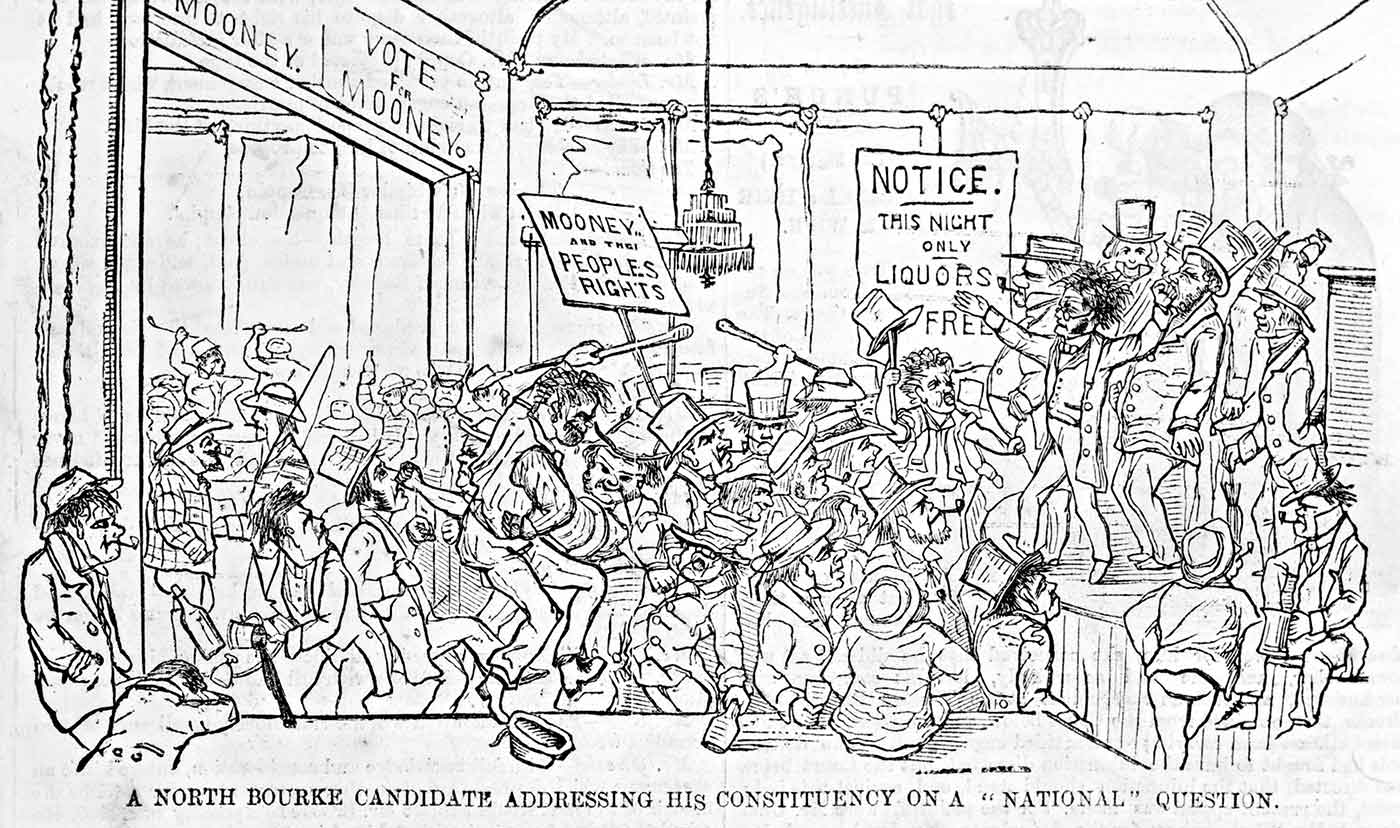
\includegraphics[scale=0.25]{NorthBourke.jpg}
	\caption{Election held in 1855 in Victoria, Australia 
	  was conducted in pub!}
	\end{center}
  \end{figure}   
  


%% Chapters
\chapter{Background}
\label{cha:background}
%At the begging of each chapter, please introduce the motivation and high-level
%picture of the chapter. You also have to introduce sections in the
%chapter. 


\section{Electronic Voting}
   Electronic voting is a nightmare because of a minuscule possibility of 
   bug in software used in voting could lead to a disaster, possibly 
   inverting the results[swisspost]. Given that the cost of 
   electronic voting is 
   so high, we should totally refrain from it; however, on contrary
   it is gaining popularity. Some of the notable countries using some form
   of electronic voting are Estonia (probably the only success story), India,
   Australia, Canada and USA. 
    \begin{figure}[htb]
	\begin{center}
	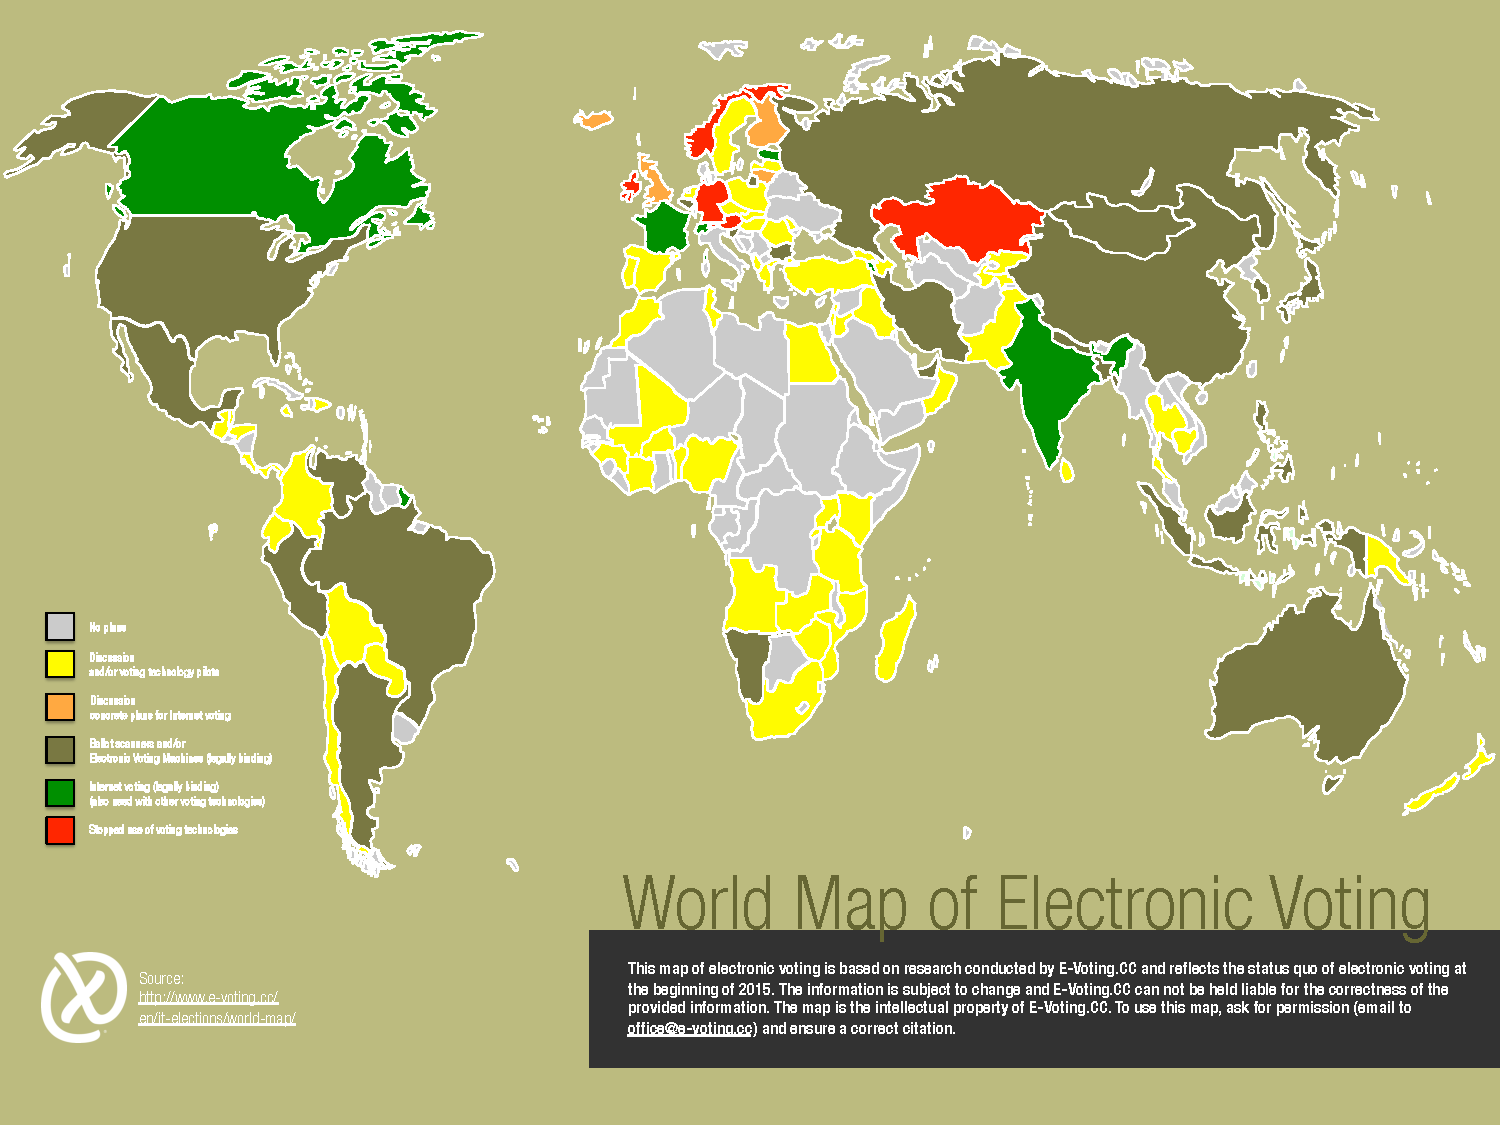
\includegraphics[scale=0.5]{e-voting_worldmap_2015.pdf}
	\caption{World map of Electronic Voting}
	\end{center}
  \end{figure}  
   
  The world can be divided into five categories on 
  parameter of electronic voting\footnote{https://www.e-voting.cc/en/it-elections/world-map}[Figure 2.1]
  \begin{itemize}
  \item No electronic voting (Grey Area)
  \item Discussion and/or voting technology pilots (Yellow Area)
  \item Discussion, concrete plans for Internet voting (Orange Area)
  \item Ballot scanners, Electronic Voting Machines, and Internet Voting
        (Green and Dark Green)
  \item Withdrawn voting technology because of public concern (Red Area)
        Germany, The Nederlands, and UK  
  \end{itemize}    
  
 

   
%  The input method, form of ballot, used the countries participating 
%  in electronic voting can be broadly divided into three group 
  Arguments in favour of electronic voting are 
  increased voter turnout, faster result and cost. Senate 
  election conducted in Western Australia in September 2013 were 
  declared void by high court because of loss of 1370 votes. It was 
  re-conducted in April 2014 with cost of 20 Million AUD with additional 
  delay in results\footnote{https://www.theguardian.com/world/2014/feb/28/western-australia-senate-election-re-run-to-be-held-on-5-april}. Sometimes, 
  the cost is not only concern, but the time involved in counting 
  is. \fix{Give a example of seat which took considerable amount 
  of time in declaring result}. 
  \fix{Add time and cost saving in Indian election after using 
  electronic voting machines} 
  The advantages of electronic voting 
  looks so promising, so why some countries (Red Area) retracted 
  from electronic voting ? Off course, electronic voting makes 
  the process faster, but it has its own layer of added complexities 
  which creates a trust issue among voters. 
  In 2005 German election, two voters filed a case in German 
  Constitutional Court (Bundesverfassungsgericht) because their 
  appeal to scrutinize the elections 
  was not heeded by the Committee. They argued that using electronic 
  voting machines to conduct the election was unconstitutional, and 
  these machines could be hacked, hence results of the 2005 election 
  could not be trusted. The case was argued on the grounds 
  of "all essential steps in the elections are subject to 
  public examinability." according to German Constitution 
  (Basic Law for the Federal Republic of Germany). 
  The Court noted that, under the constitution, elections are 
  required to be public in nature
  
  "The principle of the public nature of elections requires that all 
  essential steps in the elections are subject to public examinability
  unless other constitutional interests justify an exception. 
  Particular significance attaches here to the monitoring of the 
  election act and to the ascertainment of the election result. "
  \footnote{https://www.bundesverfassungsgericht.de/
  SharedDocs/Entscheidungen/EN/2009/03/cs20090303\_2bvc000307en.html}

  The court did not rule out or prevent the usage of electronic 
  voting machines,  but suggested to make the process more 
  transparent and trustworthy.  
  
  "The legislature is not prevented from using electronic voting machines 
  in the elections if the constitutionally required possibility of a 
  reliable correctness check is ensured. In particular, voting machines 
  are conceivable in which the votes are recorded elsewhere in addition
   to electronic storage. This is for instance possible with electronic
   voting machines which print out a visible paper report of the vote 
   cast for the respective voter, in addition to electronic recording 
   of the vote, which can be checked prior to the final ballot and is
    then collected to facilitate subsequent checking. Monitoring that is
     independent of the electronic vote record also remains possible when
     systems are deployed in which the voter marks a voting slip and the 
     election decision is recorded simultaneously, 
     or subsequently by electronic means in 
     order to evaluate these by electronic means at the end of the 
     election day."
  
  The Netherlands were among few countries who adopted electronic voting 
  in early nineties (1990), but it did not go very well long run and was 
  abolished in 2008 
  [http://www.cs.ru.nl/B.Jacobs/PAPERS/E-votingHistory.pdf]. 
  The reason for abolishing electronic voting was that   
  the voting machines used in election were susceptible to many attacks
   and could not stand 
  for public verifiability of results. The decision was victory for 
  Dutch public foundation, Wij vertrouwen stemcomputers niet
  \footnote{English Translation "We do not trust voting computers"}, which 
  demonstrated that e-voting machines used in election leaks enough
  information to guess the option, 
  and they can be easily intercepted from 20 to 30 meters
  \footnote{https://www.youtube.com/watch?v=B05wPomCjEY}. 
  
  
  Germany and The Netherlands are some of the rarest cases where 
  electronic voting was withdrawn because it was not able to 
  replicate the same trust environment as created by paper ballot.
  At this point, the reader can get into the impression that 
  countries who are using electronic voting have successfully 
  created the trust environment in electronic voting. Sadly, 
  it is not the case. India, one of the largest democracy in world, 
  uses electronic voting machines (also known as EVMs) for national 
  and state level 
  elections even though many political parties raised security 
  concern against it.
  It was already shown in 2010 in the paper 
  Security Analysis of India's Electronic Voting Machines by 
  Scott Wolchok et. al 
  [https://jhalderm.com/pub/papers/evm-ccs10.pdf] that it 
  is possible to manipulate the election results by replacing the 
  parts of machine with malicious look alike components with sending 
  them instructions over wireless
  \footnote{https://www.youtube.com/watch?v=ZlCOj1dElDY} 
  \footnote{https://indiaevm.org/}. 
  In recent elections of 2019, the Election Commission of India 
  announced, to ensure the transparency and 
  increase the trust of public, that it would use 
  voter-verified paper audit trail (VVPAT) 
  one per assembly; however, the Supreme Court of India ordered Election 
  Commission of India to increase it to five
  \footnote{https://www.news18.com/news/india/sc-directs-ec-to-increase-vvpat-verification-from-one-evm-to-five-evms-per-constituency-2093363.html}.
  The Commission  would count VVPAT slips 
  in randomly selected one polling booth per assembly 
  constituency in state election and 
  in one polling booth in each assembly segment for national election, but 
  now following the Supreme Court decision it has to do the same for 
  5 randomly selected assembly constituencies/segments. 
  \fix{Find out if there is a document at Election Commission of 
  India website and how the process works}. The design of these 
  machines are closely guard secret,  but it not impossible to gain 
  access as shown by  Scott Wolchok et. al. It would be more 
  interesting and beneficial for Indian democracy if Election 
  Commission of India
  releases the design to public scrutiny (very much like cryptographic
  implementation review process).
  
  
  
 
  
    
  
   
   \subsection{Software Bugs : Origin of Problem}
   
   
   \subsection{Estonia : Success Story}

   \subsection{Universal Verifiability}


\fix{Can I introduce Write Hilbert's idea of mathematical formalism/Frege}

A proof assistant is a computer program which assists users in development of mathematical proofs. The idea of 
developing mathematical proofs using computer goes back to Automath (automating mathematics)
[cite Automath] and LCF [cite Logic for computation] project. The 
Automath project (1967 until the early 80's)  was initiative of De Bruijn, and the aim of the project was to develop
a language for expressing mathematical theories which can be verified by aid of computer.  Automath was first 
practical project to exploit the Curry-Howard isomorphism (proofs-as-programs and formulas-as-types)
 [reference here]. DeBruijn  was likely unaware of this correspondence, and he almost re-invented it 
 ([Wiki entry on Curry-Howard]). Many researchers refers Curry-Howard isomorphism as 
 Curry-Howard-DeBruijn isomorphism. Automath project can be seen as the precursor of
 proof assistants NuPrl [cite here] and Coq [cite coq].   Some other notable  proof assistants are 
 LCF (Logic for Computable Functions)  [cite Milner?], Mizar [cite], Nqthm/ACl2 [cite], PVS [cite], 
 HOL (a family of tools derived from LCF theorem prover), Agda [cite], and Lean [cite].


In this chapter, I will give a overview of theoretical foundation of 
Coq thorem prover i.e. Calculus of Construction and  
Calculus of Inductive Construction, followed by Dependent type 
and how it leads to 
correct by construction (paradigm?) with a example of dependent 
typed lambda calculus. I will also discuss distinction between Type and Prop 
and how it affects the code extraction, a feature for extracting 
certified functional programs from specification proofs, and the 
specification language Gallina. Finally, I would 
argue that why should we trust the Coq proofs even though it does not 
match or look like a mathematical proof.



 
\section{Computer Programming and Type Theory}
	\begin{itemize}
	\item Some tracking of History about how type theory was introduced 
	     to computer programming. Use Dirk's expertise here
	\item Type theory is a logical foundation introduced by 
	      Russel to solve the problem of  paradox in Frege's 
	      Begriffsschrift.
	\item A Church invented formal system of computation, Lambda calculus
	\item A typed lambda calculus
	\item Curry Howard isomorphism
	\end{itemize}


\section{Coq: Interactive Theorem prover}
\label{sec:problemstatement}
\fix{explain here a about Coq. What is Coq ?}
The Coq proof assistant  is an interactive theorem prover based on
underlying theory of Calculus of 
Inductive Construction [Cite Pualine Mohring]  which itself is an 
augmentation of Calculus of Construction 
[cite Huet and Coquand] with inductive data-type.  
 

\subsection{Calculus of Construction}
\subsection{Calculus of Inductive Construction}
\fix{Flesh out the details of 
 Calculus of construction and Inductive construction}
 \fix{Write here about syntax and semantics of CIC}
 
 

 
\subsection{Dependent Types}
    Type system is a wide spectrum ranging from Scheme where 
    type is runtime concept to Haskell to Coq 
    
    \subsubsection{Example : Dependent Type Lambda Calculus}
     Lambda Calculus encoded in Coq using Inductive data type. 
     
 \subsubsection{Correct by Construction}
 \fix{Combing program with proofs leads to one stop solution, mainly 
     correct by construction}
  Well typed program can't go wrong. 
  Give a example of dependent type lambda calculus(Dirk's white board)
  Hello World is dependent type Vector 
 \subsubsection{Program Execution : Proof Certificate}
 \subsubsection{Type vs. Prop : Code Extraction}
 \fix{explain here the difference between Prop and Types. How it affects 
  the code extraction }
  It's good starting point to tell the reader that we have two definitions, 
  one in type and other in prop. Why ? Because Type computes, but it's
  not very intuitive for human inspection while Prop does not compute, 
  but it's very intuitive for human inspection. We have connected that 
  the definition expressed in Type is equivalent to Prop definition. 
 
 \subsubsection{Gallina : The Specification Language}
  The example, dependent type lambda calculus, I gave in previous 
  section was encoded in Coq's specification language Gallina. 
  Gallina is a highly expressive specification 
  language for development of mathematical theories and proving the    
  theorems about these  theories; however, writing proofs in Gallina
  is very tedious and cumbersome. It's not suitable for large proof 
  development, and to ease the proof development Coq also provides 
  tactics.  The user interacting with Coq theorem prover applies these 
  tactics to build the  Gallina term  which otherwise would  
  be very laborious.
  
  \fix{Can I give a simple example to demonstrate the difference 
     between proof build directly in Gallina and proof build using 
     tactics}
  
 
  

 
 \subsection{Trusting Coq proofs}
  The fundamental question for trusting the Coq proofs is two fold: 
  i) is the logic (CIC) sound ?, ii) is the implementation correct ?. 
  The logic has already been reviewed by many peers and proved correct 
  using some meta-logic. The 
  Coq implementation itself can be partitioned into two parts: 
  i) Validity Checker (Small kernel), 
  ii) Tactic language to build the proofs.
  We lay our trust in validity checker, because it's small kernel. If there
  is bug in tactic language which often is the case then build proof would 
  not pass the validity checker.  
  
  Try to write here how Fuzzer failed to find bugs in Compcert. 
  
\section{Summary} 
  Paves the path to Cryptography. 
    
\section{Cryptography}
    Write some basic crypto stuff
    
    \subsection{Homomorphic Encryption}
     Add the details of 
     homomorphic encryption 
     \subsubsection{El-Gamal Encryption Scheme}
        Give both additive and multiplicative
     \subsubsection{Pallier Encryption Scheme}
        Write some description
     \subsection{Commitment Schemes}   
        \subsubsection{Hash Based Commitment Scheme}
        \subsubsection{Discrete Logarithm Based Commitment Scheme}
         Pedersen's Commitment Scheme
     \subsection{Zero Knowledge Proof}
  		Details from 
  	 \subsection{Sigma Protocol : Efficient Zero Knowledge Proof}
  



\section{Summary}











%\label{sec:problemstatement}
Now I give a small example which defines natural number, addition of two natural numbers, and 
proof that addition over natural number is commutative.   We can define 
natural number in Coq using inductive data type (listing 1.1), addition of the natural numbers 
(listing 1.2), and proof that addition of natural numbers is commutative written in Gallina (listing 1.3).

\begin{lstlisting}[language=haskell, numbers=none, basicstyle=\ttfamily, 
caption=Inductive Data Type for Natural Numbers,  captionpos=b, xleftmargin=.1\textwidth]

Inductive Natural : Type :=
 | O : Natural
 | Succ : Natural -> Natural

\end{lstlisting}

More precisely, the interpretation is that Natural is a inductive type with two constructors: i) O representing zero,
and ii) Succ representing successor which takes a Natural number and gives next Natural number.

\fix{Change the Addition into infix symbol + and use + in proofs. It will convey the idea more clearly}
\begin{lstlisting}[language=haskell, numbers=none, basicstyle=\ttfamily,  caption=Addition function for Natural Numbers,  captionpos=b, xleftmargin=.1\textwidth]

 
Fixpoint Addition (n m : Natural) : Natural :=
  match n with
  | O => m
  | Succ n' => Succ (Addition n' m)
  end.

(* Notation for Addition. Now we can use + instead of 
   writing Addition *)
Notation "x + y" := (Addition x y)
            (at level 50, left associativity).
\end{lstlisting}

We define the addition by pattern matching on first argument \textbf{n}. When \textbf{n} is 
O (zero), then we sum is \textbf{m}, and if \textbf{n} is \textbf{Succ n'}, then sum is successor of 
\textbf{n' +  m}.

\begin{lstlisting}[language=haskell, numbers=none, basicstyle=\ttfamily,  caption=Addition function for Natural Numbers,  captionpos=b, xleftmargin=.1\textwidth]

Theorem Addition_by_zero : forall (n : Natural), n + O = n.
  refine (fix IHa (n : Natural) : n + O = n :=
            match n as nz return (nz + O = nz) with
            | O => eq_refl
            | Succ n' =>
              let IHn' := IHa n' in
              eq_ind_r (fun m => Succ m = Succ n') eq_refl IHn'
            end).
Qed.

  
Lemma Successor_addition : forall (n m : Natural),
    Succ (n + m) = n + (Succ m).
  refine
    (fix IHn (n : Natural) : forall m : Natural,
        Succ (n + m) = n + (Succ m) :=
       match n as nz return (forall m : Natural,
                                Succ (nz + m) =
                                nz + (Succ m)) with
       | O => fun m : Natural => eq_refl
       | Succ n' =>
         fun m : Natural =>
           eq_ind (Succ (n' + m))
                  (fun t => Succ (Succ (n' + m)) = Succ t)
                  eq_refl (n' + (Succ m)) (IHn n' m)
       end).
Qed.
     

    
Theorem Addition_is_commutative :
  forall (n m : Natural), n +  m = m + n.
  refine
    (fix IHn (n : Natural) : forall m : Natural,
        n + m = m + n :=
       match n as nz return (forall m : Natural,
                                nz + m =
                                m + nz) with
       | O => fun m : Natural => eq_ind_r (fun t => m = t)
                                      eq_refl
                                      (Addition_by_zero m)
       | Succ n' =>
         fun m  =>
           eq_ind (Succ (m + n'))
                  (fun t => Succ (n' + m) = t)
                  (eq_ind_r (fun t => Succ t = Succ (m + n'))
                            eq_refl (IHn n' m))
                  (m + (Succ n'))
                  (Successor_addition m n')
       end).
Qed.


\end{lstlisting}


We need two additional Lemma:
 i) $Addition\_by\_zero$, a proof of n + 0 = 0,
 and ii) $Successor\_addition$, a proof of Succ (n + m) = n + (Succ m) 
 to prove that addition on Natural is commutative ($Addition\_is\_commutative$), 
 
 One thing that can't escape from the reader's eyes is that the proofs written in Gallina is verbose, and they don't 
 appear anywhere compared to a proof that would have been written by a mathematician. Well, we can lift the burden 
 of verbosity by using tactics provided by Coq; however, there is no universally accepted solution in Coq community 
 for second problem. There has been some research in declarative style proof writing 
 \footnote{www-verimag.imag.fr/~corbinea/ftp/publis/bricks-poster.pdf}, but it is not widely practised in Coq 
 community. The proof of addition on Natural is commutative re-written using tactics (Listing 1.4)
 
 
 \begin{lstlisting}[language=haskell, numbers=none, basicstyle=\ttfamily,  caption=Addition function for Natural Numbers,  captionpos=b, xleftmargin=.1\textwidth]

Lemma Addition_by_zero : forall (n : Natural), n + O = n.
  induction n; cbn; [auto | rewrite IHn; auto].
Qed.


Lemma Successor_addition : forall (n m : Natural),
    Succ (n + m) = n + (Succ m).
Proof.
  induction n; intros m;
    cbn; [auto | rewrite <- IHn; auto].
Qed.


Theorem Addition_is_commutative :
  forall (n m : Natural), n +  m = m + n.
Proof.
  induction n; intro m;
    [rewrite Addition_by_zero |
     rewrite <- Successor_addition;
     rewrite <- IHn]; auto.
Qed.

\end{lstlisting}

Section~\ref{sec:motivation} xxxx.\\


Section~\ref{sec:relatedwork} yyyy.\\


%\section{Motivation}
%\label{sec:motivation}


%\section{Related work}
%\label{sec:relatedwork}
%You may reference other papers. For example: 
%Generational garbage collection~\citep{LH:83,Moon:84,Ungar:84} is perhaps the
%single most important advance in garbage collection since the first collectors
%were developed in the early 1960s. (doi: "doi" should just be the doi part, not
%the full URL, and it will be made to link to dx.doi.org and resolve.
%shortname: gives an optional short name for a conference like PLDI '08.)
%
%
%
%
%
%\section{Summary}
%Summary what you discussed in this chapter, and mention the story in next
%chapter. Readers should roughly understand what your thesis takes about by only reading
%words at the beginning and the end (Summary) of each chapter.




\chapter{Design and Implementation}
\label{cha:design}
Same as the last chapter, introduce the motivation and the high-level picture to
readers, and introduce the sections in this chapter.


\section{Smart Design}
\label{sec:des-hotpath}

\section{Summary}
Same as the last chapter, summary what you discussed in this chapter and
be the bridge to next chapter.

\chapter{Experimental Methodology}
\label{cha:methodology}

\section{Software platform}
\label{sec:softplat}



\section{Hardware platform}
\label{sec:hardplat}

Table~\ref{tab:machines} shows how to include tables and Figure~\ref{fig:helloworld} shows how to include codes.
\begin{table*}
  \centering
  \input table/machines.tex
  \caption{Processors used in our evaluation.}
  \label{tab:machines}
\end{table*}



\begin{figure}
  \centering
  \subfigure[\label{fig:c:hello}]{
  \begin{minipage}[b]{\columnwidth}
    \lstinputlisting[linewidth=\columnwidth,breaklines=true]{code/hello.c}\vspace*{-2ex}
  \end{minipage}}
  \subfigure[\label{fig:java:hello}]{
  \begin{minipage}[b]{\columnwidth}
    \lstinputlisting[linewidth=\columnwidth,breaklines=true]{code/hello.java}\vspace*{-2ex}
  \end{minipage}}
  \caption{Hello world in Java and C.}
  \label{fig:helloworld}
\end{figure}



%%% Local Variables: 
%%% mode: latex
%%% TeX-master: "paper"
%%% End: 

\chapter{Results}
\label{cha:result}




\section{Direct Cost}\
\label{sec:direct_cost}

Here is the example to show how to include a figure. Figure~\ref{fig:cost}
includes two subfigures (Figure~\ref{fig:zerocost}, and Figure~\ref{fig:zerobus});

\begin{figure*}
  \label{fig:cost}
  \subfigure[Fraction of cycles spent on zeroing\label{fig:zerocost}]{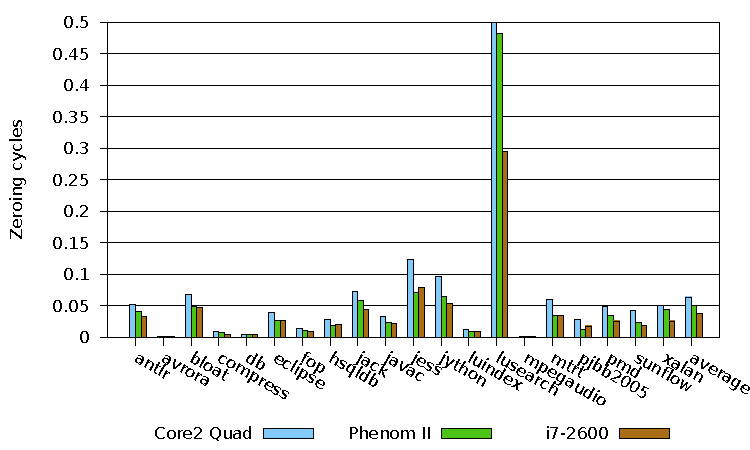
\includegraphics[width=\columnwidth]{figs/zerocost_intel.pdf}}
  \subfigure[BytesZeroed / BytesBurstTransactionsTransferred\label{fig:zerobus}]{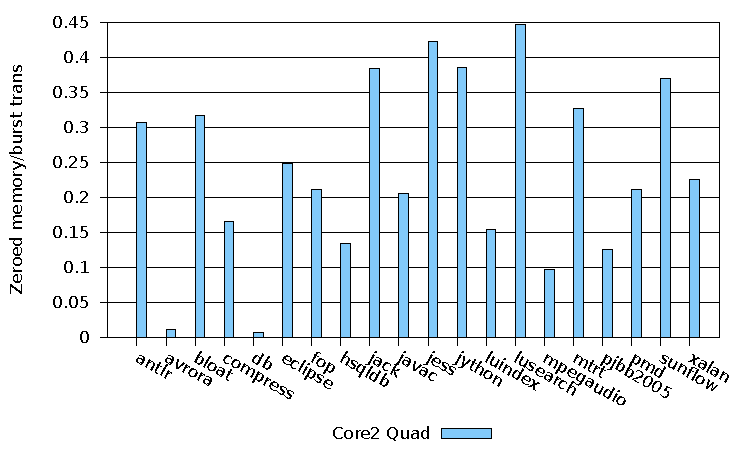
\includegraphics[width=1.0\columnwidth]{figs/zerobus_core.pdf}}
  \caption{The cost of zero initialization}
\end{figure*}


\section{Summary}

\chapter{Conclusion}
\label{cha:conc}
Summary your thesis and discuss what you are going to do in the future in Section~\ref{sec:future}.


\section{Future Work}
\label{sec:future}
Good luck.





%%%%%%%%%%%%%%%%%%%%%%%%%%%%%%%%%%%%%%%%%%%%%%%%%%%%%%%%%%%%%%%%%%%%%%
% Here begins the end matter

%%% \appendix

\backmatter

\bibliographystyle{anuthesis}
\bibliography{thesis}

\printindex

\end{document}
